\documentclass[11pt]{article}

\usepackage{amsmath}
\usepackage{amssymb}
\usepackage{graphicx}
\usepackage{caption}
\usepackage{subcaption}

\topmargin -.5in
\textheight 9in
\oddsidemargin -.25in
\evensidemargin -.25in
\textwidth 7in

\newcommand{\code}[1]{\texttt{#1}}

\begin{document}

\author{Gu, Qiao}
\title{16-720B Homework 3 Write-up}
\maketitle

\medskip

\subsection*{Q1.1}

\newcommand{\W} {\mathcal{W}}
\newcommand{\I} {\mathcal{I}}
\newcommand{\B} {\mathcal{B}}
\newcommand{\w} {\mathbf{w}}
\newcommand{\x} {\mathbf{x}}
\newcommand{\p} {\mathbf{p}}
\newcommand{\A} {\mathbf{A}}

\begin{itemize}
  \item $\frac{\partial \W(\x; \p)} {\partial \p^T}$ is the graident of the warped coordinates over the warping parameter $\p$, which is:
  \begin{align} \label{warp_gradient_translation}
      \frac{\partial \W(\x; \p)} {\partial \p^T} =
      \frac{\partial \x + \p} {\partial \p^T} =
      \begin{bmatrix}
          1 & 0 \\
          0 & 1
      \end{bmatrix}.
  \end{align}

  \item For the iterative process, replace $\p$ with $\p+\Delta \p$ in Eq. (2) of the handout, and then

  \begin{align} \label{ls}
      \I_{t+1}(\x+\p+\Delta \p) - \I_t(\x)
      &= \I_{t+1} (\x + \p) + \frac{\partial \I_{t+1}(\x+\p)}{\partial(\x+\p)^T} \Delta \p - \I_t(\x) \\
      &= \nabla \I_{t+1}(\x+\p) \Delta \p - (\I_t(\x) - \I_{t+1} (\x+\p)).
  \end{align}

  Therefore the Eq. 2 of the handout in vector form is (Note that each $\nabla \I_{t+1}(\x+\p)$ are of shape $1\times2$.)

  \begin{align} \label{eq:q1.1LS}
      \arg\min_{\Delta \p}
      \left \|
      \begin{bmatrix}
          \nabla \I_{t+1}(\x_1+\p) \\
          \nabla \I_{t+1}(\x_2+\p) \\
          \cdots\\
          \nabla \I_{t+1}(\x_D+\p)
      \end{bmatrix}
      \Delta \p -
      \begin{bmatrix}
          \I_t(\x_1) - \I_{t+1} (\x_1+\p)\\
          \I_t(\x_2) - \I_{t+1} (\x_2+\p)\\
          \cdots\\
          \I_t(\x_D) - \I_{t+1} (\x_D+\p)\\
      \end{bmatrix}
      \right \|
      =
      \arg\min_{\Delta \p}
      \| \A\Delta\p - \mathbf{b} \|
  \end{align}

  The big matrix and the big vector on the L.H.S. of the above equation are the $\A$ and $\mathbf{b}$.

  \item To solve for the least square solution of Eq.~\ref{eq:q1.1LS}, we need to compute $(\A^T\A)^{-1}\A^T\mathbf{b}$. Therefore, we must have $\A^T\A$ to be invertible.
\end{itemize}

\newpage
\subsection*{Q1.3}

Please find the results of Lucas-Kanade tracking results in Figure.~\ref{fig:q1.3}

\begin{figure}[h!]
    \begin{subfigure}{.19\textwidth}
      \centering
      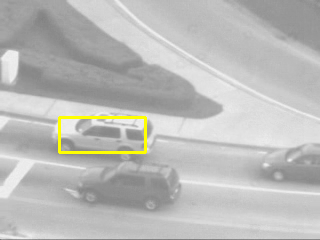
\includegraphics[width=.95\linewidth]{../results/carseqrects_0.png}
      \caption{frame 1}
    \end{subfigure}
    \begin{subfigure}{.19\textwidth}
      \centering
      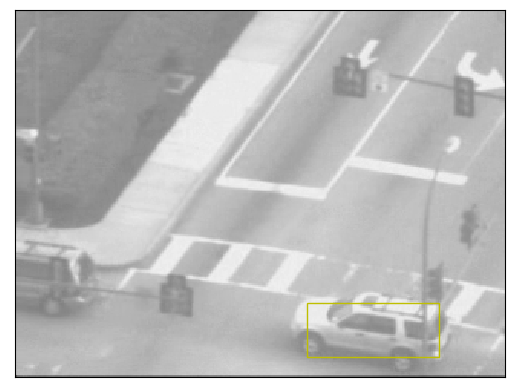
\includegraphics[width=.95\linewidth]{../results/carseqrects_99.png}
      \caption{frame 100}
    \end{subfigure}
    \begin{subfigure}{.19\textwidth}
      \centering
      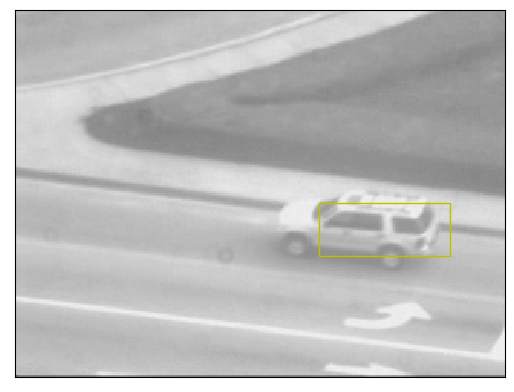
\includegraphics[width=.95\linewidth]{../results/carseqrects_199.png}
      \caption{frame 200}
    \end{subfigure}
    \begin{subfigure}{.19\textwidth}
      \centering
      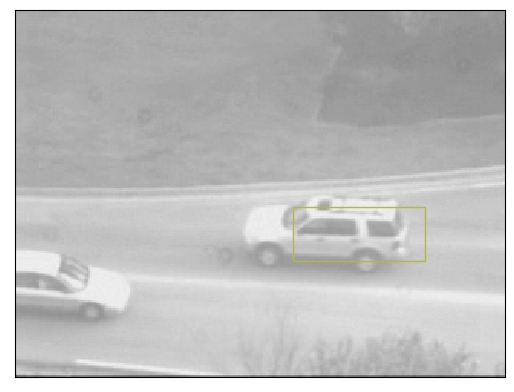
\includegraphics[width=.95\linewidth]{../results/carseqrects_299.png}
      \caption{frame 300}
    \end{subfigure}
    \begin{subfigure}{.19\textwidth}
      \centering
      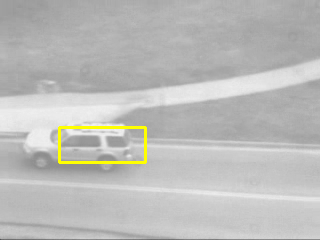
\includegraphics[width=.95\linewidth]{../results/carseqrects_399.png}
      \caption{frame 400}
    \end{subfigure}\hfill
    \caption{Lucas-Kanade Tracking Results with One Single Template. }
    \label{fig:q1.3}
\end{figure}

\newpage
\subsection*{Q1.4}




\end{document}
